\section{Worlds, world states, and their transformations}\label{sec:A mathematical treatment of worlds and their transformations}

%%%%%%%%%%%%%%%%%%%%%%%%%%%%%%%%%%%%%%%%%%%%%%
\subsection{What is the most general form of a world?}
\newthought{A world consists} of \emph{world states}, which are how the world is at a snapshot in time, and a way to move between world states when the world changes; we call a change of a world from one world state to another a \emph{transformation}.

Mathematically, we can represent the collection of world states as a set $W$ of objects, the collection of transformations as a set $D$ of objects that connect world states; individual world states in $W$ and individual transformations in $D$ are distinguishable in some way\footnote{
We are building up to using our framework to consider the transformation structure of the world from the perspective of an agent. So when we say \emph{distinguishable in some way} we mean that there is some way for our agent to distinguish between the world states or the transformations.
}.
We connect transformations with their associated world states using a source map
\begin{equation}
	s: D \to W,
\end{equation}
which sends each transformation to the world state it originates at, and a target map
\begin{equation}
	t: D \to W,
\end{equation}
which sends each transformation to the world state it ends at.
Note that we haven't enforced any structure on the world states or the transformations except that each transformation connects two world states.

\begin{notation}
	We denote a transformation $d \in D$ with a source of $w$ and a target of $w'$ as $d: w \to w'$.
\end{notation}

These source and target maps allow us to represent a world as a type of graph $\mathscr{W}$ with arrows (the transformations in $D$) connecting vertices (the world states $W$).
Since it is possible to have a world where more than one transformation has the same source and the same target, our graph $\mathscr{W}$ must be a \emph{multigraph}.
Since it is possible to have a world where there is a transformation from a world state $w$ to a world state $w'$, but not have a transformation from $w'$ back to $w$\footnote{In other words, a world with an irreversible change.}, our multigraph $\mathscr{W}$ must be \emph{directed}.
A multigraph that is directed is called a \emph{multidigraph}.

\begin{postulate}
	The most abstract mathematical representation of a world is a multidigraph that consists of a collection $W$ of world states as vertices, a collection $D$ of transformations as arrows, a source map $s$ that maps each arrow to the world state it is leaving, and a target map $t$ that maps each arrow to the world state it is entering.
\end{postulate}

\begin{notation}
    We denote a world $\mathscr{W}$ with a set $W$ of world states, a set $D$ of transformations, a source map $s$ and a target map $t$ by
    \begin{equation}
        \mathscr{W} = (W, D, s, t).
    \end{equation}
\end{notation}

%%%%%%%%%%%%%%%%%%%%%%%%%%%%%%%%%%%%%%%%%%%%%%
\subsection{Constructing worlds from atomic transformations}

\begin{postulate}
	All transformations are made up of sequences of \emph{atomic transformations}, which cannot be broken down into smaller transformations.
\end{postulate}

We will construct our world $\mathscr{W}$ from atomic transformations\footnote{
Note that, in a similar same way as for distinguishable world states, when we use our framework to describe the representation of an agent, these atomic transformations can be thought of as the transformations giving the smallest change to an aspect of a world state that is detectable by the agent.
}, but first we will establish some properties of atomic transformations.

\begin{notation}
    We use a $\hat{ }$ symbol to explicitly denote that something is atomic, contains atomic things, or that an operator acts exclusively on atomic things.
\end{notation}

Let $\hat{D}$ be the set of atomic transformations.
We define atomic source and target maps
\begin{equation}
	\hat{s}: \hat{D} \to W \quad\quad \hat{t}: \hat{D} \to W
\end{equation}
such that for any atomic transformation $\hat{d} \in \hat{D}$
\begin{equation}
	\hat{d}: w \to w' \implies \hat{s}(d) = w \text{ and } \hat{t}(d) = w'.
\end{equation}

Using $W$, $\hat{D}$, $\hat{s}$, and $\hat{t}$ we can construct another multidigraph $\hat{\mathscr{W}}$, which we call the \emph{atomic multidigraph of the world}
\begin{equation}
	\hat{\mathscr{W}} = (W, \hat{D}, \hat{s}, \hat{t}).
\end{equation}

Our set $D$ of all transformations of $\mathscr{W}$ is the set of all finite directed walks in $\mathscr{W}$\footnote{
    The atomic transformations are in $D$ as directed walks of length 1.

    $D$ is countably infinite if $\hat{\mathscr{W}}$ contains directed cycles, since walks can traverse cycles repeatedly to generate walks of arbitrary length.
    If $\hat{\mathscr{W}}$ is acyclic (contains no directed cycles), then $D$ is finite.
    If we had defined $D$ as the set of all directed walks (not just finite directed walks), then $D$ would have been uncountably infinite.
}.
This means that a transformation $d \in D$ is a sequence of atomic transformations\footnote{
	Composition of transformations is read from right to left.
}
\begin{equation}
	d = \hat{d}_{n} \hat{\circ} \hat{d}_{n-1} \hat{\circ} ... \hat{\circ} \hat{d}_{1}
\end{equation}
where
\begin{equation}
	\hat{\circ}: \hat{D} \times \hat{D} \to D
\end{equation}
is the \emph{atomic transformation composition operator} that is defined if\footnote{
This operator $\hat{\circ}$ is the operator of concatenation of directed walks of length 1.
}
\begin{equation}
	\hat{t}(\hat{d}_{i}) = \hat{s}(\hat{d}_{i+1}) \quad \text{for $i = 1, ..., n-1$}.
\end{equation}

\begin{corollary}
    The composition operator $\hat{\circ}$ is associative\footnote{
    An operator $\cdot$ is \emph{associative} if it satisfies
    \begin{equation}
    	a \cdot (b \cdot c) = (a \cdot b) \cdot c.
    \end{equation}
    This means that when we perform the operation $\cdot$ on three or more elements, the way in which the elements are composed does not affect the outcome.
    }
    by the definition of concatenation of directed walks.
\end{corollary}

%%%%%%%%%%%%%%%%%%%%%%%%%%%%%%%%%%%%%%%%%%%%%%%%%%%%%%%%%
\paragraph{Trivial transformations.}

\newthought{For each world state} $w \in W$ of our multidigraph $\hat{\mathscr{W}}$, there is a trivial walk that does not leave $w$.
We call the associated transformation of this trivial walk the \emph{trivial transformation at $w$} and denote it by $1_{w}$\footnote{
Trivial transformations essentially represent no transformation happening in the world.
}.
Therefore, for all $w \in W$, there exists a trivial transformation $1_{w} \in D$ with the following properties
\begin{align}
	\hat{s}(1_{w}) = w \\
	\hat{t}(1_{w}) = w.
\end{align}
Trivial walks serve as neutral elements in the concatenation of directed walks, and so transformation sequences involving trivial transformations are not distinct elements in $D$ (except for the sequences of containing only a single trivial transformation); for example, $\hat{d} \circ 1_{s(d)}$ is the same element in $\hat{D}$ as $\hat{d}$.
In other words, trivial transformations satisfy
\begin{align}
	& \hat{d} \circ 1_{\hat{s}(\hat{d})} = \hat{d} \quad \text{for all $\hat{d} \in \hat{D}$} \\
	& 1_{\hat{t}(\hat{d})} \circ \hat{d} = \hat{d} \quad \text{for all $\hat{d} \in \hat{D}$}.
\end{align}
We denote the set of trivial transformations by
\begin{equation}
	D_{\varepsilon} = \{ 1_{w} \mid w \in W \}.
\end{equation}

\paragraph{Extending from $\hat{\mathscr{W}}$ to $\mathscr{W}$.}
\newthought{Each transformation in} $D$ can now be uniquely expressed as a sequence of composed atomic transformations or as a single trivial transformation:
\begin{equation}
    \operatorname{Seq} : \left\{ 
    \begin{array}{l}
        D \backslash D_{\varepsilon} \to (\hat{D})^{n} \\
        D_{\varepsilon} \to D_{\varepsilon}
    \end{array} \right.
\end{equation}
such that
\begin{align}
    & \operatorname{Seq}(d) = (\hat{d}_{n}, \hat{d}_{n-1}, \dots, \hat{d}_{1}) \quad \text{for $d = \hat{d}_{n} \hat{\circ} \hat{d}_{n-1} \hat{\circ} \dots \hat{\circ} \hat{d}_{1}$} \\
    & \operatorname{Seq}(1_{w}) = 1_{w} \quad \text{for all $w \in W$}.
\end{align}

We can extend our atomic source map $\hat{s}$ and atomic target map $\hat{t}$ to our source map $s$ and target map $t$ as, for a transformation $d \in D$ with $\operatorname{Seq}(d) = (\hat{d}_{n}, \hat{d}_{n-1}, \dots, \hat{d}_{1})$,
\begin{align}
	& s(d) = \hat{s}(\hat{d}_{1}) \\
	& t(d) = \hat{t}(\hat{d}_{n}).
\end{align}

We can also extend the atomic transformation composition operator $\hat{\circ}$ to the \emph{transformation composition operator} on the entire set $D$ as:
\begin{equation}
\begin{aligned}
	& \circ: D \times D \to D \\
	& \text{where $d' \circ d$ is defined if $t(d) = s(d')$}
\end{aligned}
\end{equation}
such that, for $\operatorname{Seq}(d) = (\hat{d}_{n}, \hat{d}_{n-1}, \dots, \hat{d}_{1})$ and $\operatorname{Seq}(d') = (\hat{d'}_{m}, \hat{d'}_{m-1}, \dots, \hat{d'}_{1})$
\begin{equation}
	\operatorname{Seq}(d' \circ d) = (\hat{d'}_{m}, \hat{d'}_{m-1}, \dots, \hat{d'}_{1}, \hat{d}_{n}, \hat{d}_{n-1}, \dots, \hat{d}_{1}).
\end{equation}

\begin{corollaryE}
    $\circ$ is associative by the definition of concatenation of directed walks\footnote{
        $\circ$ is the operator of concatenation of directed walks.
        We can now naturally extend stuff like the neutral element condition for trivial transformations as
        \begin{align}
            & d \circ 1_{s(d)} = d \quad \text{for all $d \in D$} \\
            & 1_{t(d)} \circ d = d \quad \text{for all $d \in D$}.
        \end{align}
    }.
\end{corollaryE}


\begin{notation}
	When defining a world $\mathscr{W}$ it is sufficient to give $W$ and $\hat{D}$ since we can always construct $D$ from $\hat{D}$.
	We also usually don't explicitly provide the source and target maps when defining a world.
\end{notation}


\paragraph{Length of a transformation.}
\newthought{The \emph{length} $|d|$ of} a transformation $d \in D$ is the number of atomic transformations that make up its associated directed walk in $\hat{\mathscr{W}}$ \footnote{
    This means that
    \begin{align}
        & |d| = 1 \quad \text{for all $d \in \hat{D}$} \\
        & |1_{w}| = 0 \quad \text{for all $1_{w} \in D_{\varepsilon}$}.
    \end{align}
}.

%%%%%%%%%%%%%%%%%%%%%%%%%%%%%%%%%%%%%%%%%%%%%%
\subsection{Simplifications}

\newthought{We make the} following simplifications to worlds in our framework.


\paragraph{Deterministic worlds.}
\newthought{In a \emph{deterministic}} world, every change in the current world state has a single guaranteed effect.
A world that is not deterministic is called \emph{stochastic}; in a stochastic world, the same change to the current world state could produce different results.
We will initially consider deterministic worlds.


\paragraph{Discrete worlds.}
\newthought{In a \emph{discrete}} world, the number of states and the number of transformations between states are countable.
A world that is not discrete is called \emph{continuous}.
For simplicity, we only consider discrete worlds.
However, we can make the following argument that it is actually more natural to consider discrete worlds than continuous worlds.
Consider a continuous world $\mathscr{W}$ and an agent with $n$ sensors $\theta_{i}$ that can produce a sensor observation $o_{i}$ of $\mathscr{W}$ as
\begin{equation}
	\theta_{i}(w) = o_{i}
\end{equation}
where $i \in \{1, ..., n\}$ and $w \in W$.
We hypothesis that there are transformations that cause changes to their source world state that are so small that the changes cannot be perceived by the agent; in other words, there exist transformations $d \in D$ such that
\begin{equation}
	\theta_{i}(s(d)) = \theta_{i}(t(d)).
\end{equation}
Such transformations do not exist from the perspective of the agent; therefore, from the perspective of the agent there will be discrete jumps between perceptible world states\footnote{
From this perspective, a world forms a sort of directed discrete manifold; we can sometimes approximate this to a sort of directed continuous manifold.
}.
We will initially consider discrete worlds.

%%%%%%%%%%%%%%%%%%%%%%%%%%%%%%%%%%%%%%%%%%%%%%%%%%%%%
\subsection{World diagrams}

\newthought{We can visually} represent the structure of our multidigraphs using \emph{world diagrams} consisting of dots for the world states and arrows for the transformations.
These diagrams can make it easier to visualise and understand the structure and properties of a world.

Since our set $D$ is very large\footnote{
	If we have transformations $d: s(d) \to t(d)$ and $d': s(d) \to t(d)$, then we can construct sequences like $d' \circ d$, $d' \circ d \circ d' \circ d$ etc..., which means $D$ has an infinite number of elements:
	\begin{center}
		\FloatBarrier
		\captionsetup{type=figure}
		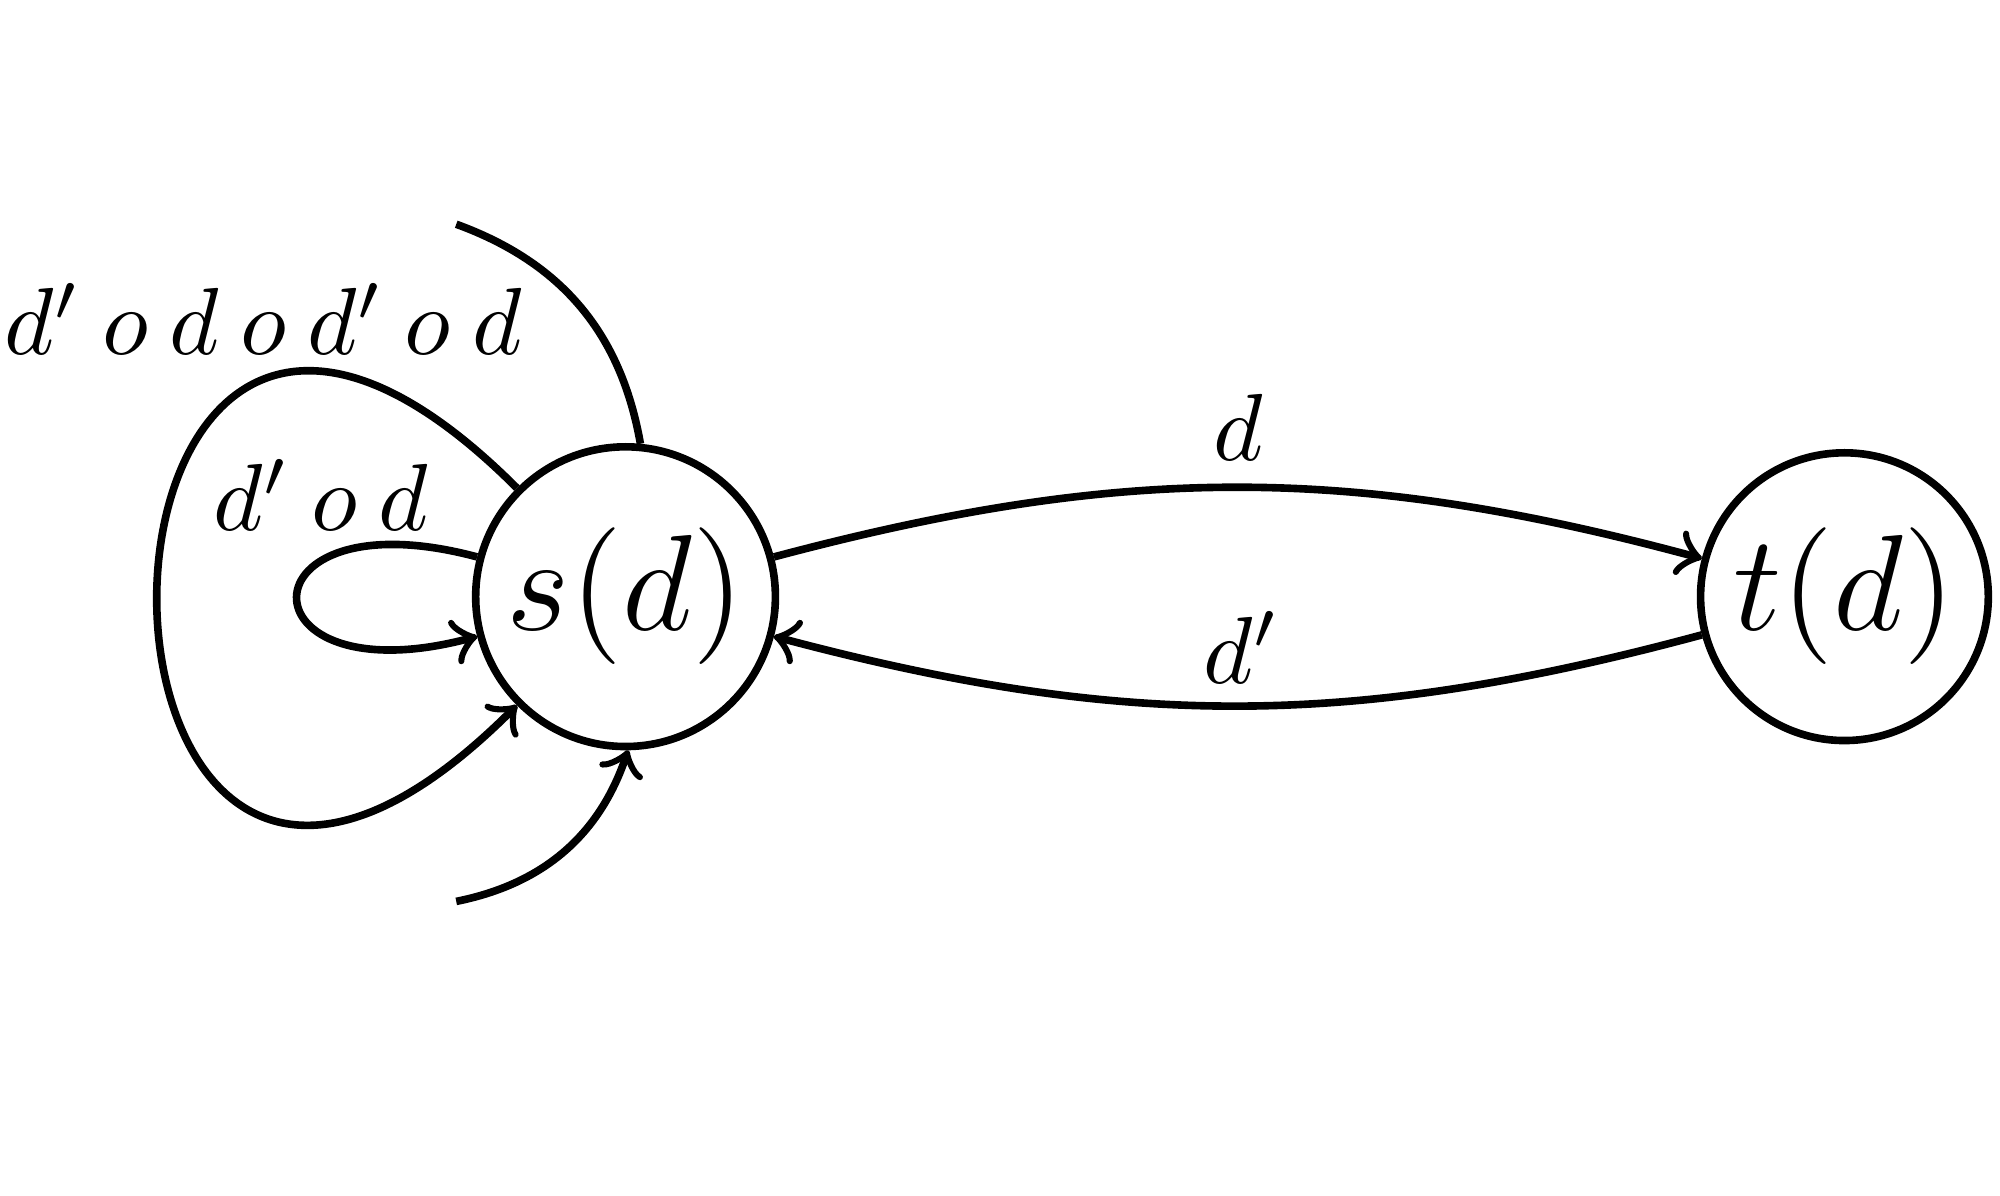
\includegraphics[width=1.0\linewidth]{2MathematicalFramework/Images/D_commonly_large.png}
		% \captionof{figure}{Test caption.}
		\caption{A world diagram showing sequences of the transformations $d$ and $d'$ that are of the form $(d' \circ d)^{n}$.}
	\end{center}
}, we do not show all the transformations in $D$ in our world diagrams unless explicitly stated.
When drawing the world diagram for a world $\mathscr{W}$, we default to drawing the vertices and arrows of the atomic multidigraph $\hat{\mathscr{W}}$ and the trivial transformations in $D_{\varepsilon}$.

\newthought{Let's look at} some world diagrams show casing some of the properties we've already seen.
\draftnote{blue}{Consider}{
Put these in the margin as we go, then say something about how these are the sort of diagrams we mean ?
}

\begin{figure}[H]
	\centering
	\begin{subfigure}[b]{0.45\linewidth}
		\centering
		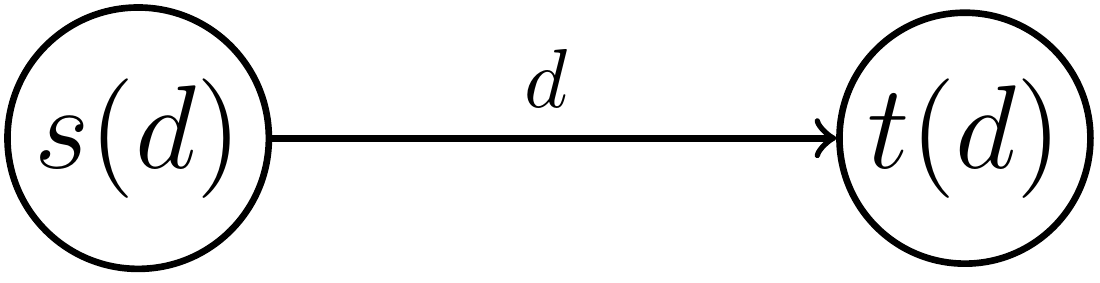
\includegraphics[width=\linewidth]{2MathematicalFramework/Images/transformation.png}
		\caption{A world diagram showing a transformation.}
		\label{fig:transformation}
	\end{subfigure}
	\hfill
	\begin{subfigure}[b]{0.45\linewidth}
		\centering
		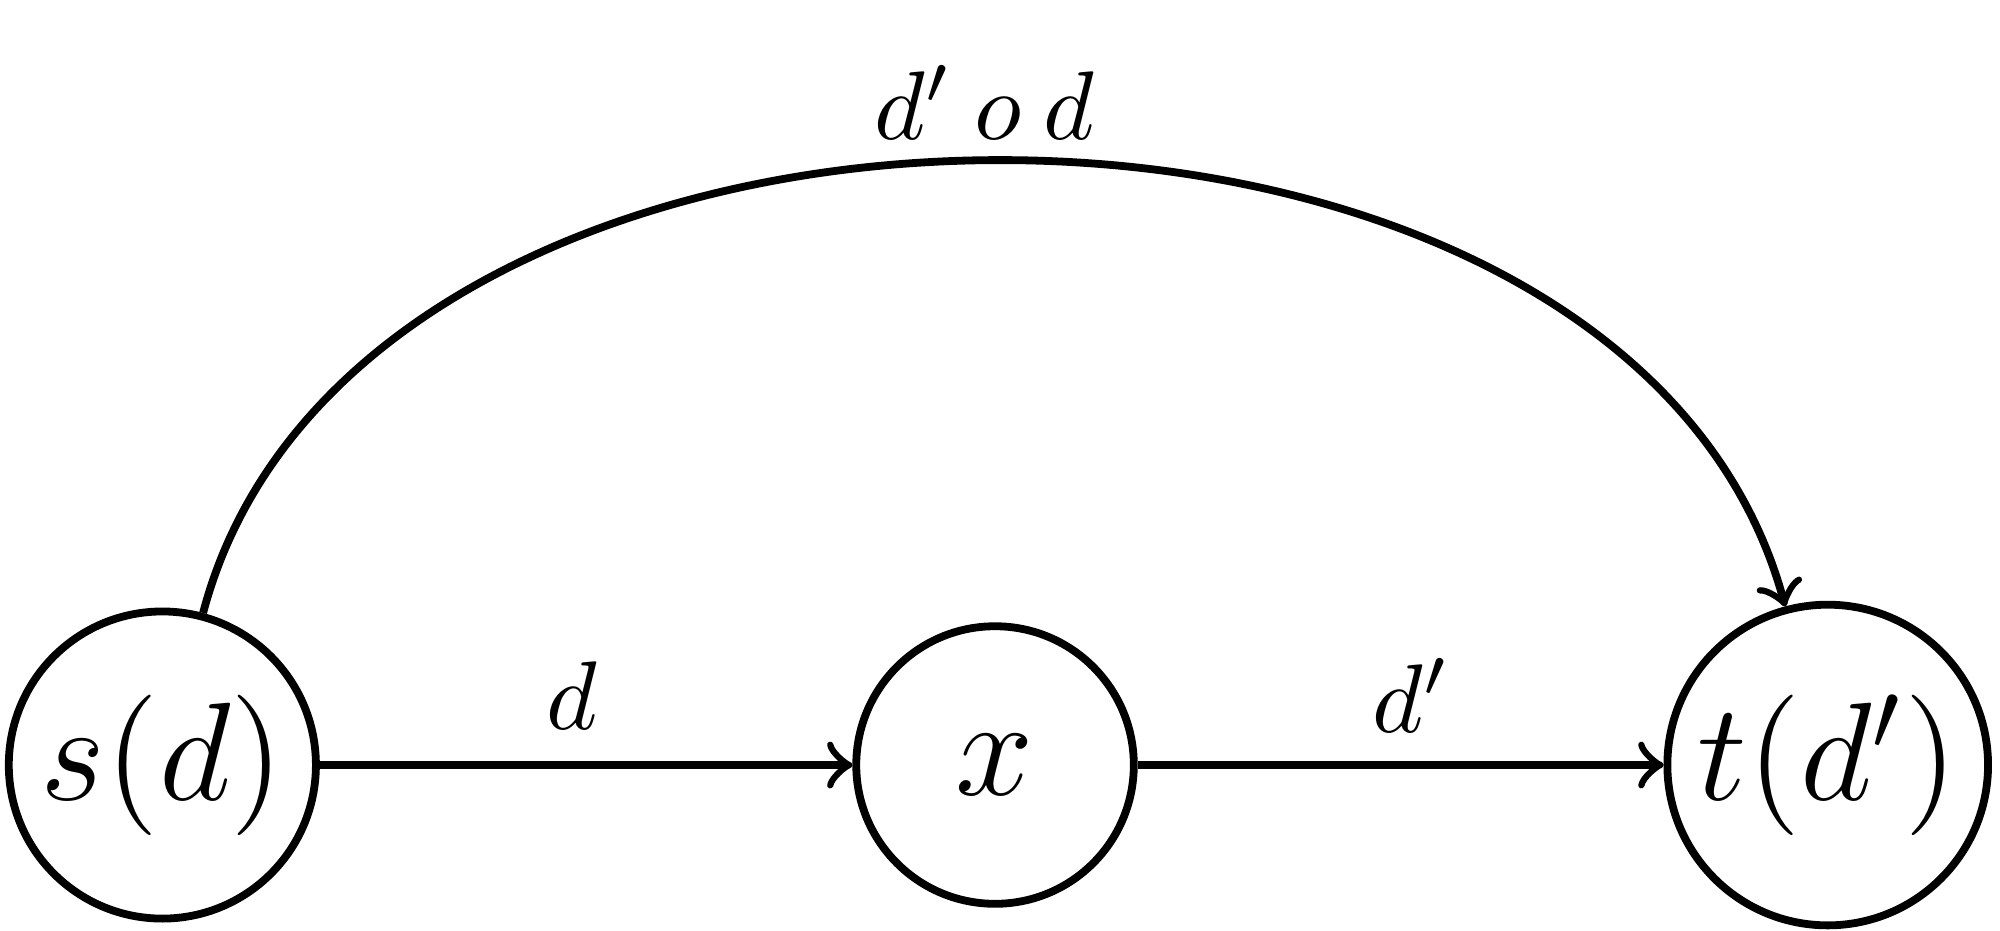
\includegraphics[width=\linewidth]{2MathematicalFramework/Images/transformation_composition.png}
		\caption{A world diagram showing the composition of two transformations $d$ followed by $d'$ to give a transformation $d' \circ d$.}
		\label{fig:transformation_composition}
	\end{subfigure}
	\vskip\baselineskip
	\begin{subfigure}[b]{0.45\linewidth}
		\centering
		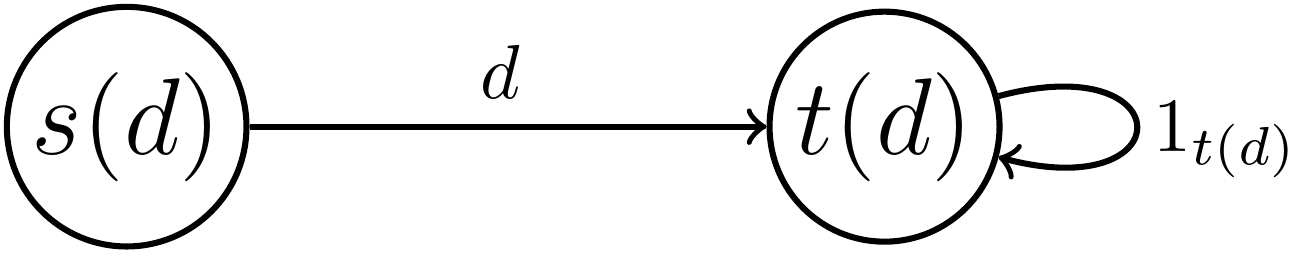
\includegraphics[width=\linewidth]{2MathematicalFramework/Images/left_trivial_transformation.png}
		\caption{A world diagram showing a transformation $d: s(d) \to t(d)$ and its left identity element, the trivial transformation $1_{t(d)}$. Composing these two transformations gives the transformation $d$.}
		\label{fig:left_trivial_transformation}
	\end{subfigure}
	\hfill
	\begin{subfigure}[b]{0.45\linewidth}
		\centering
		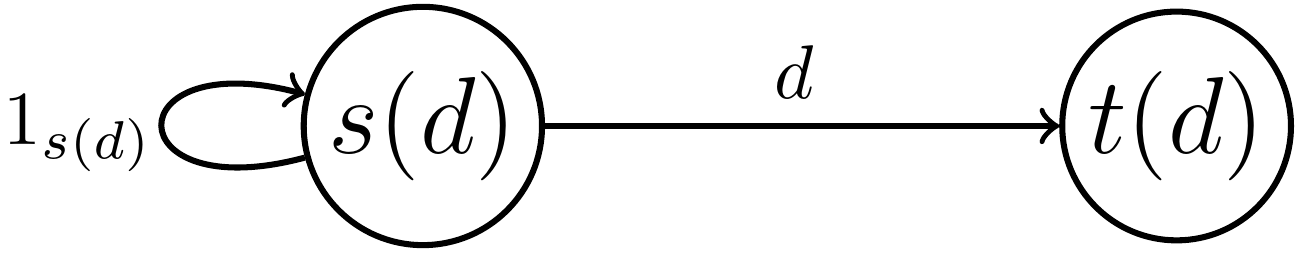
\includegraphics[width=\linewidth]{2MathematicalFramework/Images/right_trivial_transformation.png}
		\caption{A world diagram showing a transformation $d: s(d) \to t(d)$ and its right identity element, the trivial transformation $1_{s(d)}$. Composing these two transformations gives the transformation $d$.}
		\label{fig:right_trivial_transformation}
	\end{subfigure}
	\vskip\baselineskip
	\begin{subfigure}[b]{0.45\linewidth}
		\centering
		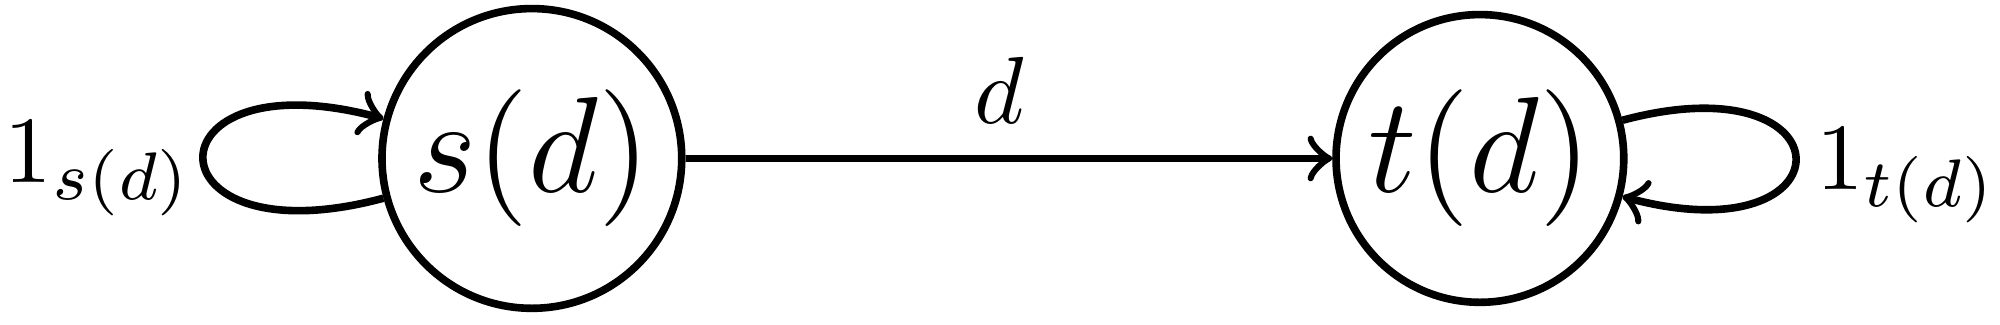
\includegraphics[width=\linewidth]{2MathematicalFramework/Images/trivial_transformations_example_all_transformations.png}
		\caption{A world diagram showing a transformation $d: s(d) \to t(d)$, its left identity $1_{t(d)}$, and its right identity $1_{s(d)}$.}
		\label{fig:trivial_transformations_example_all_transformations}
	\end{subfigure}
	\caption{Examples of world diagrams displaying some of the concepts we have already come across.}
\end{figure}

It's important to note that, in a world diagram, the positioning (relative or absolute) of the world states and the shapes and lengths of the arrows do not matter:
\begin{figure}[H]
    \centering
    \begin{tikzpicture}
        \node (left) {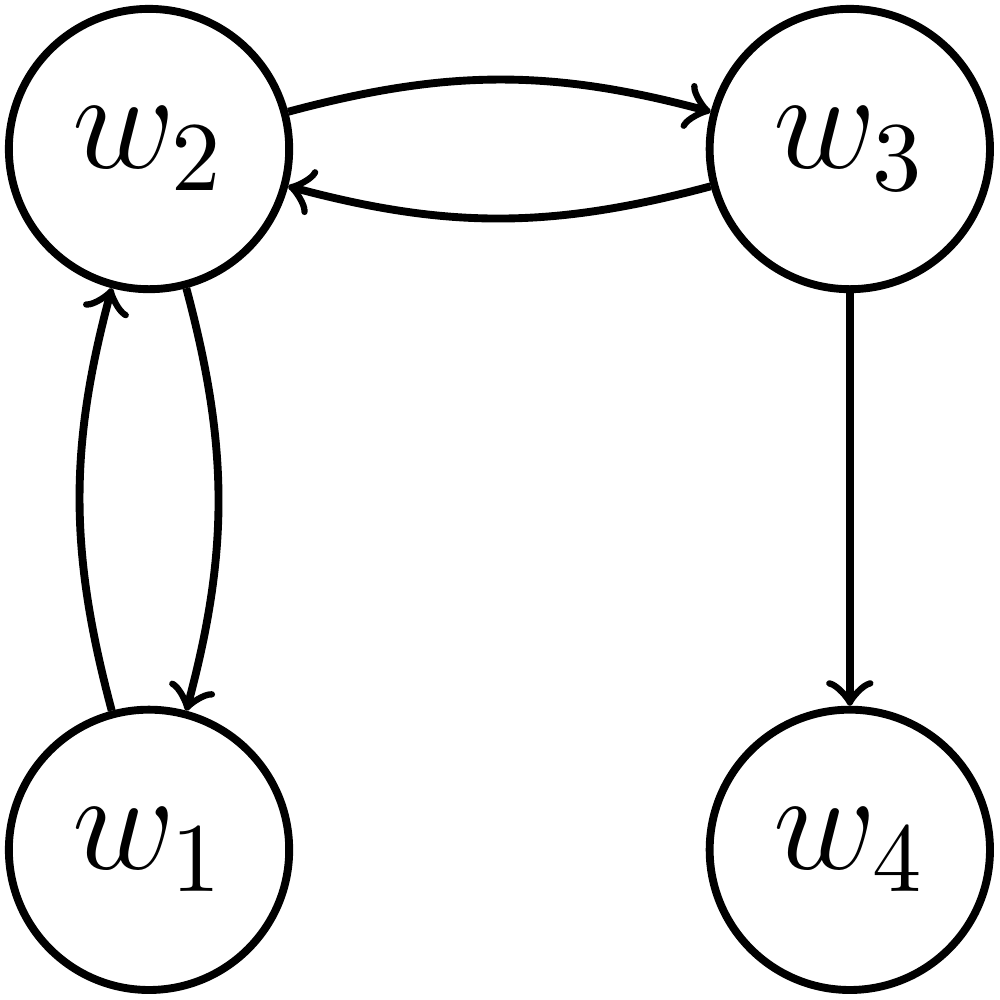
\includegraphics[width=0.3\textwidth]{2MathematicalFramework/Images/isomorphic_world_diagrams_1.png}};
        \node (sim) [right=1cm of left] {\Huge$\cong$};
        \node (right) [right=1cm of sim] {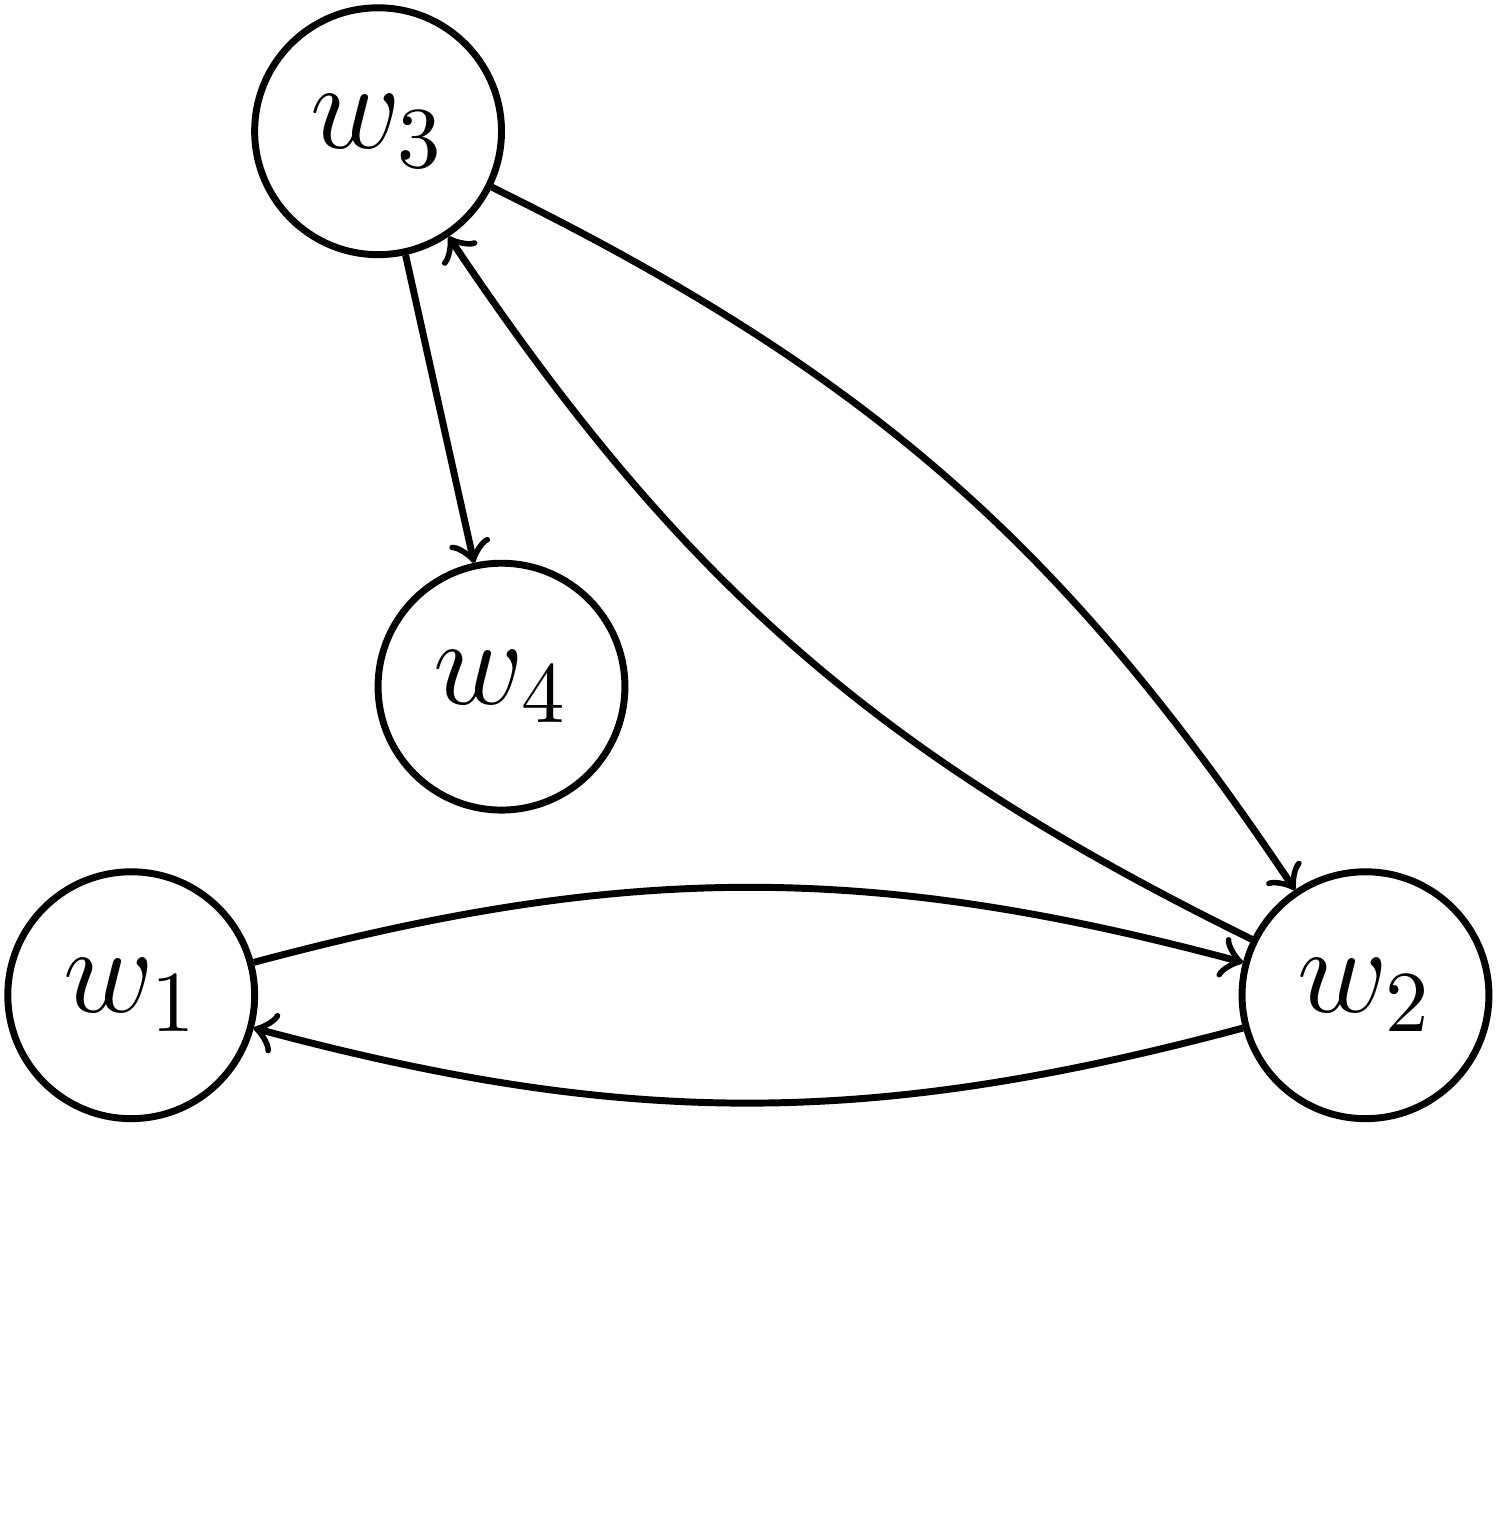
\includegraphics[width=0.4\textwidth]{2MathematicalFramework/Images/isomorphic_world_diagrams_2.png}};
    \end{tikzpicture}
    \caption{
    The properties of these world diagrams are identical (the world diagrams are isomorphic).
    }
    \label{fig:isomorphic_world_diagrams}
\end{figure}

%%%%%%%%%%%%%%%%%%%%%%%%%%%%%%%%%%%%%%%%%%%%%%%%%
\subsection{Subworlds}

\newthought{We are building} towards describing the structure of transformations in an agent's representation; later we will only be interested in the perspective of the agent and so will only care about the world states and transformations that the agent can interact with.
Reachable and unreachable subworlds give us the language to describe and then disregard parts of worlds that agents will never explore and therefore are not relevant to the agent's representation.
For example, if an agent is in a maze and a section of the maze is inaccessible from the position that the agent is in, then that section of the maze would be disconnected from the section of the maze that the agent is in; if we want to study how the agent’s representation evolves as it learns, it makes sense to disregard world states where the agent is in the inaccessible part of the maze since those world states can never be reached and so those world states will not affect the agent's representation.
\footnote{
	But what about worlds that are unreachable from the current world state, but the agent has already visited?
	If we assume the representation evolution process is Markov, then all the necessary information will contained in the current representation space of the agent and so past world states which are now unreachable are irrelevant.
	Therefore, for a Markov representation evolution process, we only need to consider the world states in subworlds that are reachable from the current world state.

	If the representation evolution process is not Markov, we can transform the representation evolution process into a Markov process by augmenting the state space of the process to include any relevant historical information.
}


\newthought{When constructing a} subworld we want to preserve the composition $\circ$, so that a subworld is a world; this means we have to be careful which transformations we remove to form a valid subworld.
A world $\mathscr{W}' = (W', D', s', t')$ is a \emph{subworld} of a world $\mathscr{W} = (W, D, s, t)$ if
\begin{enumerate}
    \item $W' \subseteq W$;
    \item $D' \subseteq D$ such that:
    \begin{enumerate}
        \item For all $d \in D'$, $s(d) \in W'$ and $t(d) \in W'$;
        \item For all $d, d' \in D'$ with $d: s(d) \to t(d)$ and $d': t(d) \to t(d')$, $d \circ d' \in D'$;
        \item For all $w' \in W'$, $1_{w'} \in D'$;
    \end{enumerate}
    \item $s'$ is the restriction of $s$ to $D' \to W'$;
    \item $t'$ is the restriction of $t$ to $D' \to W'$\footnote{
    We usually use $s$, $t$ instead of explicitly defining the maps $s'$ and $t'$ because $s$ and $t$ act on all the elements of $D$ and $D'$ is a subset of $D$.
    }.
\end{enumerate}

\begin{notation}
    If $\mathscr{W}'$ is a subworld of $\mathscr{W}$ then we can write $\mathscr{W}' \subseteq \mathscr{W}$.
\end{notation}

If $\mathscr{W}' \subseteq \mathscr{W}$, then the atomic multidigraph of $\mathscr{W}'$ is not necessarily a sub-multidigraph of the atomic multidigraph of $\mathscr{W}$; in other words, $\mathscr{W}' \subseteq \mathscr{W}$ does not necessarily mean $\hat{D}' \subseteq \hat{D}$. For example, if $\hat{d}_{1}, \hat{d}_{2} \in \hat{D}$ and $\operatorname{Seq}(d_{3}) = (\hat{d}_{2}, \hat{d}_{1})$, it is possible to have a subworld where $\hat{d}_{1}, \hat{d}_{2} \centernot\in D'$ (and so $\hat{d}_{1}, \hat{d}_{2} \centernot\in \hat{D}'$) but have $d_{3} \in D$.
In this case, $d_{3}$ would be an atomic transformation in $\mathscr{W}'$ (i.e., $d_{3} \in \hat{D}'$).\footnote{
\begin{figure}[H]
    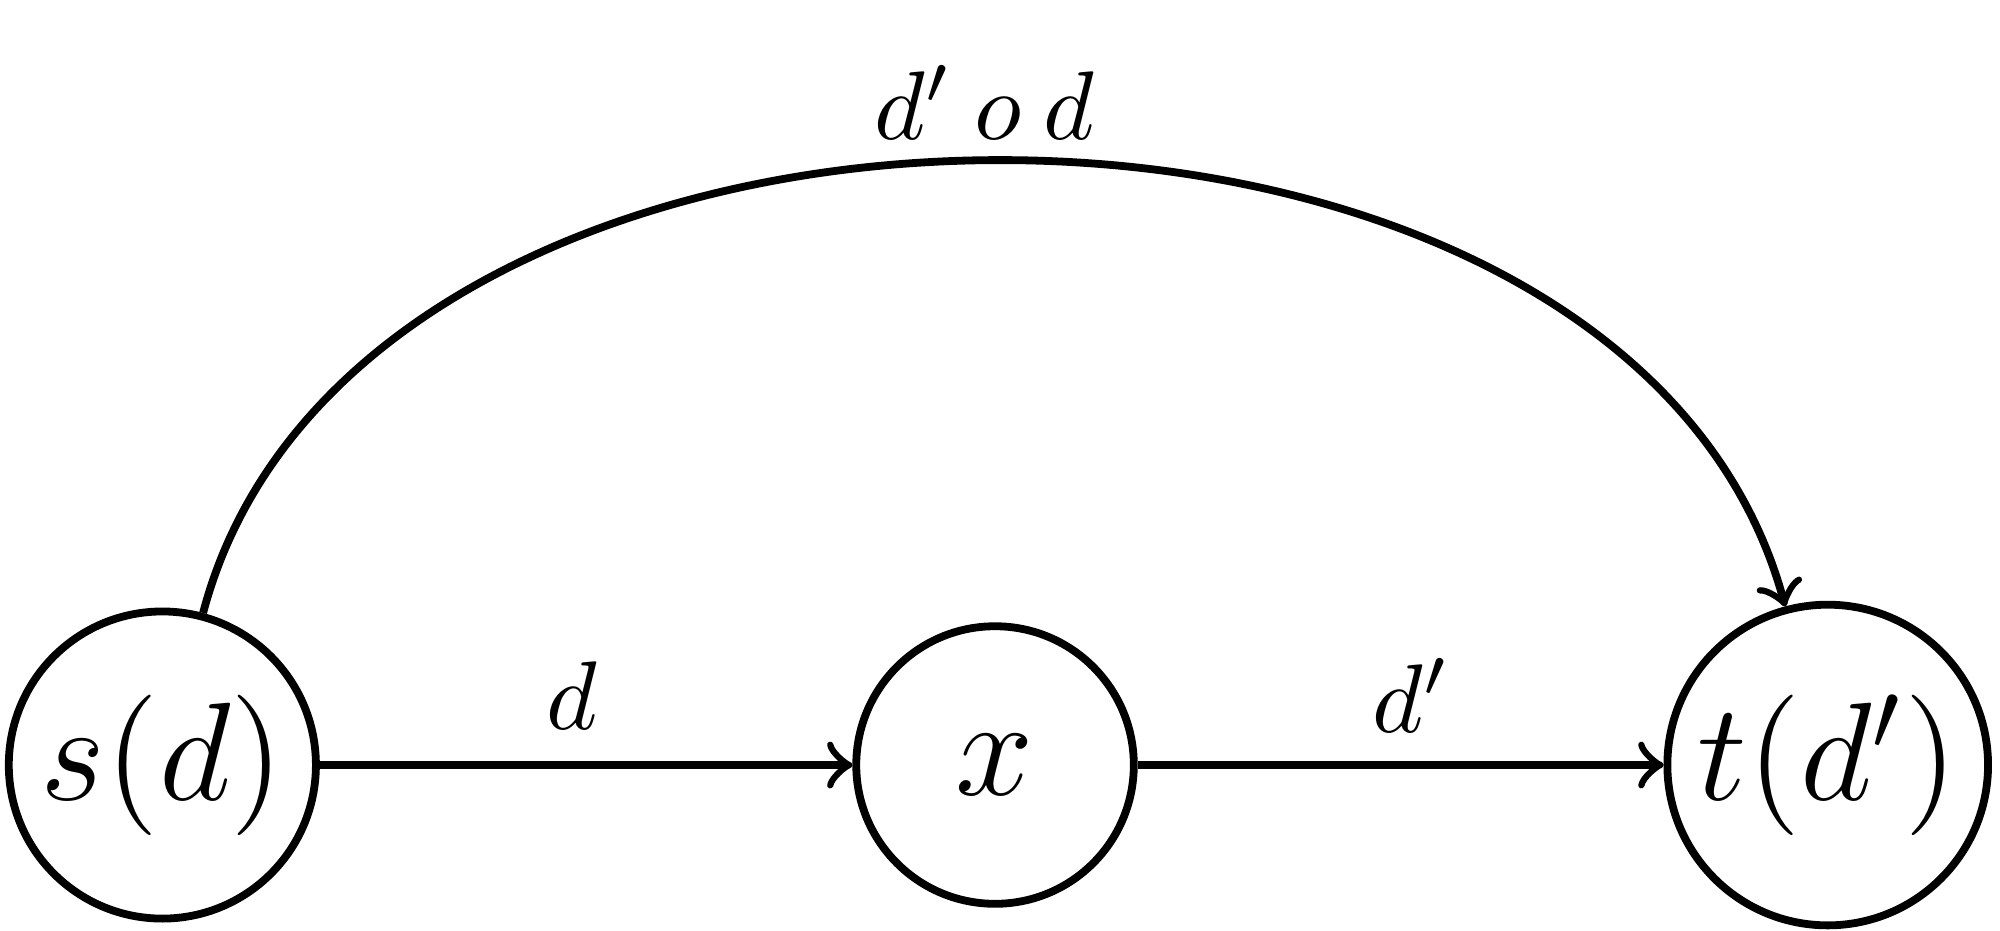
\includegraphics[width=0.5\linewidth]{2MathematicalFramework/Images/transformation_composition.png}
    \caption{
    If $d_{3} = d_{2} \circ d_{1}$ and $d_{1}, d_{2} \in \hat{D}$, then when constructing a subworld we can remove $d_{1}$ and $d_{2}$ and keep $d_{3}$ (in which case $d_{3}$ would be an atomic transinformation in the subworld), but we cannot remove $d_{3}$ without removing $d_{1}$ and $d_{2}$.
    }
\end{figure}
}
More generally, suppose $\mathscr{W}' \subseteq \mathscr{W}$; for $d \in D$ and $\operatorname{Seq}(d) = (\hat{d}_{n}, \hat{d}_{n-1}, \dots, \hat{d}_{1})$, if $\hat{d}_{n}, \hat{d}_{n-1}, \dots, \hat{d}_{1} \centernot\in \hat{D}'$, then either $d \in \hat{D}'$ or $d \centernot\in D$.
\draftnote{purple}{PS: Consider}{Is this a proposition we need to prove ?}
\footnote{
This property of subworlds allows us to construct discrete worlds out of continuous worlds by, for example, removing atomic transformations that cannot be perceived by an agent.
}
When constructing subworlds from a world, if removing atomic transformations causes another transformation to become an atomic transformation in the subworld, the number of atomic transformations in the subworld will decrease.
Therefore, we have
\begin{equation}
    \mathscr{W}' \subseteq \mathscr{W} \implies |\hat{D}'| \leq |\hat{D}|
\end{equation}
\draftnote{purple}{PS: Consider}{Is this a proposition that we need to prove ?}


%%%%%%%%%%%%%%%%%%%%%%%%%%%%%%%%%%%%%%%%%%%%%%%%%
\paragraph{Reachable and unreachable subworlds.}
\newthought{Consider a world} $\mathscr{W}^{\aleph}$ containing two subworlds $\mathscr{W}$ and $\mathscr{W}'$.
The subworld $\mathscr{W}'$ is \emph{reachable} from the subworld $\mathscr{W}$ if there exists a transformation $d \in D^{\aleph}$ with $d: w \to w'$ where $w \in W$ and $w' \in W'$.\footnote{
\begin{figure}[H]
	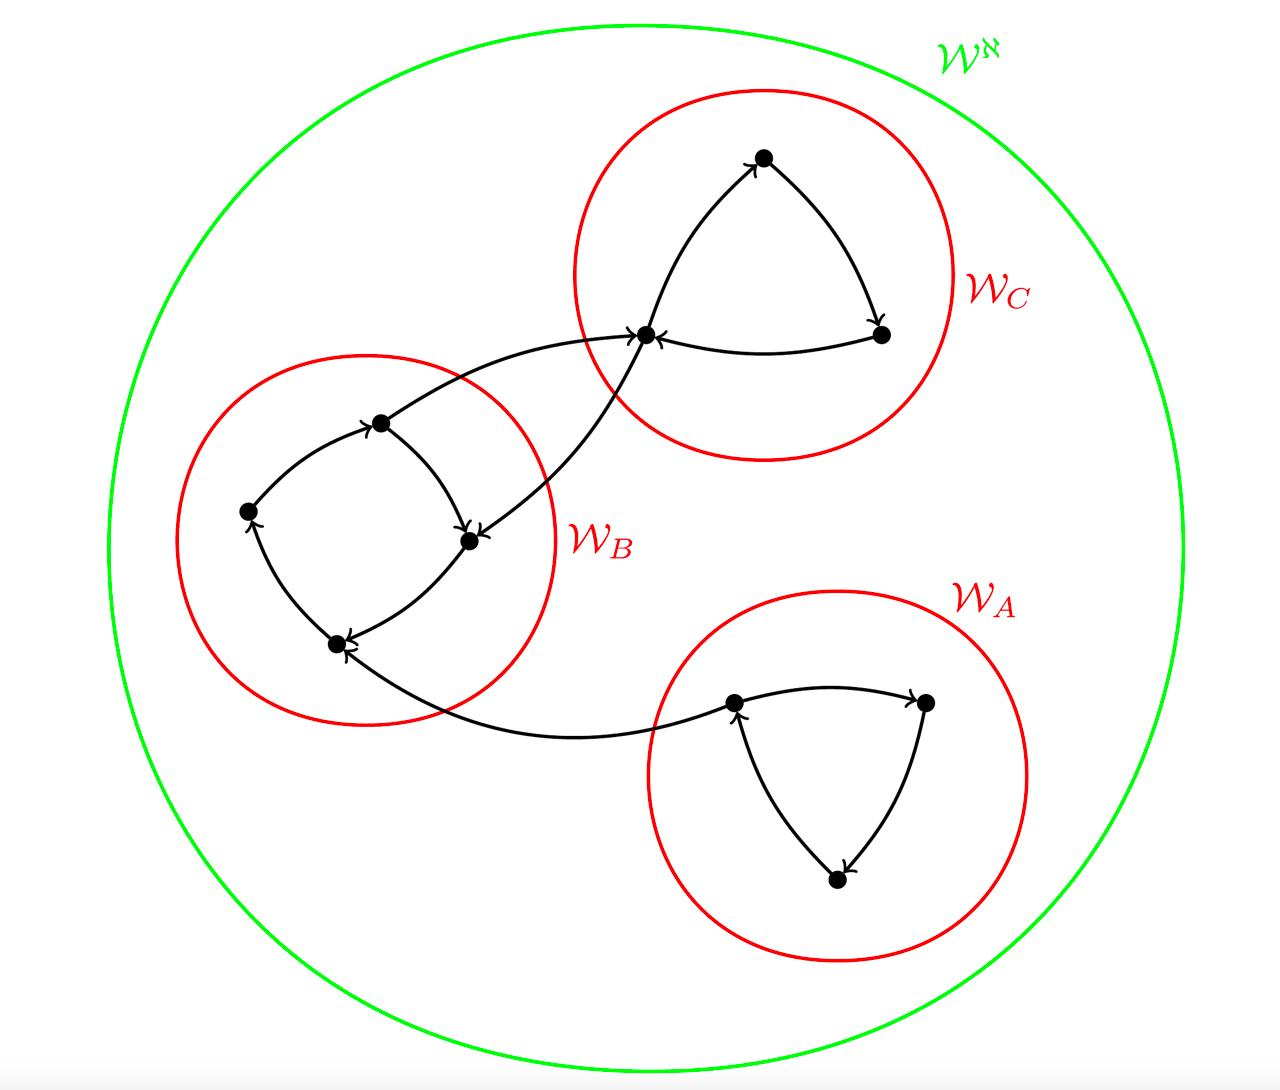
\includegraphics[width=0.5\linewidth]{2MathematicalFramework/Images/reachable_worlds.jpeg}
	\caption{
		$\mathscr{W}_{C}$ is reachable from $\mathscr{W}_{A}$ and $\mathscr{W}_{B}$, but $\mathscr{W}_{A}$ is not reachable from $\mathscr{W}_{B}$ or $\mathscr{W}_{C}$.
	}
	\label{fig:reachable_worlds}
\end{figure}
}
If a subworld is not reachable, we say it is \emph{unreachable}.

Formally, for a world $\mathscr{W} = (W, \hat{D}, s, t)$, the set of world states that are reachable from a world state $w$ is given by
\begin{equation}
	W^{\to}(w) := \{ w' \in W \mid \text{ there exists } d \in D \text{ with } d: w \to w' \}.
\end{equation}
The set of atomic transformations that are reachable from $w$ is given by\footnote{
	This is the largest subset of atomic transformations that stay within the set of reachable states.
}
\begin{equation}
	\hat{D}^{\to}(w) := \{ \hat{d} \in \hat{D} \mid s(\hat{d}) \in W^{\to}(w) \; \text{and} \; t(\hat{d}) \in W^{\to}(w) \}
\end{equation}

The atomic multigraph of the \emph{reachable subworld} of a world $\mathscr{W}$ from the state $w$ is given by
\begin{equation}
	\hat{\mathscr{W}}^{\to}(w) := (W^{\to}(w), \hat{D}^{\to}(w), s \big|_{D^{\to}(w)}, t \big|_{D^{\to}(w)})
\end{equation}
The reachable subworld $\mathscr{W}^{\to}(w)$ of $\mathscr{W}$ from the state $w$ is then constructed using $\hat{\mathscr{W}}^{\to}(w)$ in the usual way.

\begin{notation}
	We denote the current world state by $w^{*}$.
\end{notation}

The subworld that is reachable from the current world state $w^{*}$ is called the \emph{natural reachable subworld}, which we denote by $\mathscr{W}^{\to}(w^{*})$.
